\section{Introduction}\label{sec:intro}

Groups that search together find good answers faster than individuals searching apart, and they pay for it in
what they find: seeing what others have found speeds the climb, and it narrows the search. In a field
experiment on a computational biology problem, \citet{boudreau2015open} found that letting competitors see one
another's intermediate solutions raised average performance but concentrated the field on a few approaches,
while withholding solutions until the end produced more varied attempts and the best final solutions. Systems
of several LLM agents working on one problem are now common, and many of them let the agents see what the
others have done, for example through one document everyone writes to, messages between agents, or a log of
attempts and scores \citep{du2023improving,park2023generative,park2026scaling,qu2026coral,yan2025beyond}.
The usual assumption is that more visibility is better, because an agent that can see a teammate's good
result need not rediscover it. Recent work supports that assumption for problems where feedback ranks
partial progress correctly: \citet{park2026scaling} show that $k$ agents sharing a workspace beat the best of
$k$ independent agents when an agent-accessible verifier can tell better partial solutions from worse ones,
and that the advantage disappears where feedback cannot rank intermediate solutions.

A long line of work on organisational learning predicts the opposite for a different kind of problem.
\citet{march1991exploration} argued that mutual learning in a group raises short-run performance and lowers
long-run performance, because members converge on whatever currently looks best before anyone has found
what is actually best. \citet{lazer2007network} showed in simulation that well-connected groups solving a
rugged problem reach a good solution quickly and a worse solution eventually than sparsely connected groups,
and human experiments find the same pattern when the problem has a hidden better region
\citep{mason2012collaborative,derex2016partial}. The difference is the shape of the landscape. When feedback
is a reliable guide to the top, sharing lets the group climb faster. When the top is separated from the
starting point by a valley, sharing lets the group agree faster on the wrong hill. Which of the two describes
a team of LLM agents?

This paper answers that question on a task of the second kind. We use a reimplementation of
the lemonade-stand game of \citet{ederer2013pay} (Figure~\ref{fig:overview}A), originally a laboratory experiment on how pay schemes affect
human exploration. An agent runs a stand for \NRounds{} rounds. Each round it picks a location, two recipe
settings, a colour and a price, receives a profit, and reads one line of customer feedback about one of the
settings. Profit is a deterministic function of the distance between the chosen setup and a hidden ideal
setup at that location. The location the agent is pointed to at the start pays about half of what the best
location can pay, and reaching the best location requires changing the location and several settings at once,
which pays poorly until the ideal setup for that location is found. Profit is therefore an honest verifier of the current round
and a misleading guide to where the best round is. The task is a structured bandit whose arms are full setups,
with a good arm that is easy to refine and a better arm that is hard to find. The two things a team might want
from it, the best arm and the lowest regret, are measured separately.

\begin{figure}[t]
  \centering
  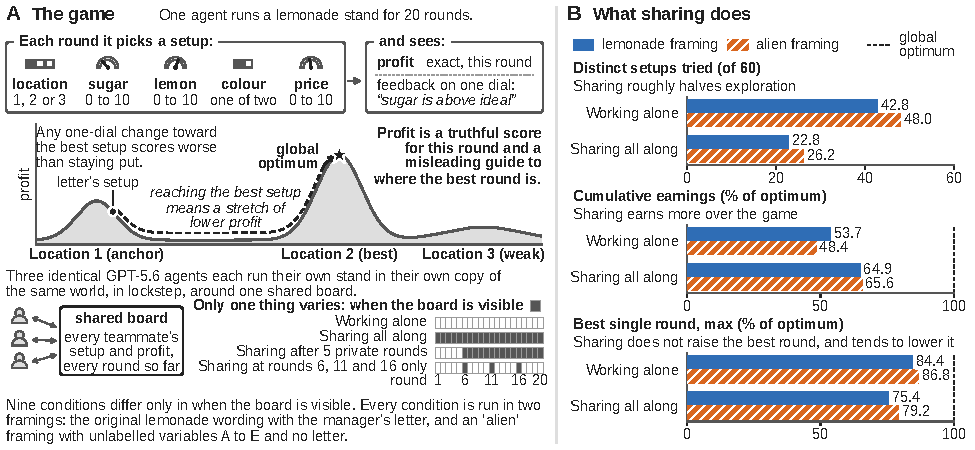
\includegraphics[width=\linewidth]{figures/fig_overview.pdf}
  \caption{\textbf{(A) The game.} An agent chooses a location and four settings each round and receives that round's profit and one line of feedback about one setting. Each location has a hidden ideal; the location the letter points to pays about half of the best one, and reaching the best one means scoring worse for a while. Three agents play the same world; conditions differ only in when the shared board of teammates' setups and profits is visible. \textbf{(B) What sharing does.} Sharing roughly halves the number of distinct setups a team tries, raises what the team earns over the game, and does not raise the best single round any teammate reaches. Means over eight worlds, GPT-5.6; blue is the lemonade framing, orange the alien framing.}
  \label{fig:overview}
\end{figure}

We put \NAgents{} identical GPT-5.6 agents in the same hidden world and vary one thing: when the shared board,
listing every teammate's setup and profit so far, is visible. Each agent is told to maximise the overall
performance of the business and nothing more. Nine conditions range from agents that never
see each other, through boards that open after two, five, ten or fifteen private rounds, to a board visible in
only three rounds, a board with an instruction to stay different from one's teammates, and agents that move
one at a time within each round. To check that the result is not an artefact of the lemonade wording and of
the recommended starting setup, every condition is also run in an alien framing, in which the same worlds are
described as five unlabelled decision variables with no recommendation. Each condition is run on
\NWorlds{} worlds, two or three times per world, so that we can report whether the first run's numbers
reproduce.

We show three things that hold in both framings. First, sharing collapses exploration
(Figure~\ref{fig:overview}B): a team that sees the
board from round one tries about half as many distinct setups as three agents working alone, and the later
the board opens, the more the team explores. This is the most reliable result in the paper: it holds in every
world, in every run and in both framings. Second, sharing raises cumulative earnings over the \NRounds{}
rounds in every sharing condition, because agents copy whoever is currently doing best and copying pays in
the current round. Third, sharing lowers the best single-round profit any teammate reaches. The size of the
drop is similar in the first run and in the repeats, but with \NWorlds{} worlds it is not statistically
reliable, and we say so. The sharing conditions that come closest to working alone on the best round are those
that preserve exploration: a board that opens late or in only three rounds, and the stay-different
instruction. Nothing we ran puts sharing reliably above working alone on the best round. A direct test of the
three-round board on sixteen further worlds puts it within a few points of working alone in both framings, and
a replication of three conditions on Claude
Opus 5.5 reproduces the exploration and earnings results, with the drop in the best round appearing in the
lemonade framing but not in the alien framing. A 60-round version of the two main conditions shows that the
trade is horizon-dependent in a way that turns on the letter: given time, sharing teams that start from a
common recommendation leave it and lose nothing on the best round while earning more, whereas teams with no
recommendation stay below working alone on the best round and keep a smaller earnings lead.

The contribution is a clean testbed and a measured answer. The testbed is small, deterministic, cheap to
run, and has a known global optimum in every world. This separates the two things a team might want: the
ceiling it reaches and the total it earns on the way. The answer is that for LLM agents on a landscape with a
valley, visibility trades the ceiling for the total, the mechanism is reduced search, and the lever that
restores the ceiling is limiting how often or how closely the agents look at each other. Section~\ref{sec:related}
places the study, Section~\ref{sec:method} describes the game, the framings, the conditions and the
measures, Section~\ref{sec:results} reports the results and their reproducibility, and
Section~\ref{sec:discussion} states what we think is established, what is not, and what we plan next.
